\let\negmedspace\undefined
\let\negthickspace\undefined
\documentclass[journal]{IEEEtran}
\usepackage[a5paper, margin=10mm, onecolumn]{geometry}
%\usepackage{lmodern} % Ensure lmodern is loaded for pdflatex
\usepackage{tfrupee} % Include tfrupee package

\setlength{\headheight}{1cm} % Set the height of the header box
\setlength{\headsep}{0mm}     % Set the distance between the header box and the top of the text

\usepackage{gvv-book}
\usepackage{gvv}
\usepackage{cite}
\usepackage{amsmath,amssymb,amsfonts,amsthm}
\usepackage{algorithmic}
\usepackage{graphicx}
\usepackage{textcomp}
\usepackage{xcolor}
\usepackage{txfonts}
\usepackage{listings}
\usepackage{enumitem}
\usepackage{mathtools}
\usepackage{gensymb}
\usepackage{comment}
\usepackage[breaklinks=true]{hyperref}
\usepackage{tkz-euclide} 
\usepackage{listings}
% \usepackage{gvv}                                        
\def\inputGnumericTable{}                                 
\usepackage[latin1]{inputenc}                                
\usepackage{color}                                            
\usepackage{array}                                            
\usepackage{longtable}                                       
\usepackage{calc}                                             
\usepackage{multirow}                                         
\usepackage{hhline}                                           
\usepackage{ifthen}                                           
\usepackage{lscape}
\begin{document}

\bibliographystyle{IEEEtran}
\vspace{3cm}

\title{3-3.2-27}
\author{AI24BTECH11015 - Harshvardhan Patidar}
 \maketitle
% \newpage
% \bigskip
{\let\newpage\relax\maketitle}

\renewcommand{\thefigure}{\theenumi}
\renewcommand{\thetable}{\theenumi}
\setlength{\intextsep}{10pt} % Space between text and floats



\numberwithin{equation}{enumi}
\numberwithin{figure}{enumi}
\renewcommand{\thetable}{\theenumi}

Question: \\
	Draw a right triangle $ABC$ in which $BC = 12$ cm, $AB = 5$cm and $\angle B = 90^{\degree}$.\\ \\


\solution\\
	 \begin{table}[h!]    
      		\centering
      		\begin{tabular}[12pt]{ |c| c|}
    \hline
    \textbf{Variable} & \textbf{Description}\\
    \hline
	$\vec{m}$ & Unit Vector\\
    \hline
	$\alpha$ & Angle of the unit vector with $x$-axis\\
    \hline
	$\beta$ & Angle of the unit vector with $y$-axis\\
    \hline	
    \end{tabular}

      		\caption{}
	\end{table}\\

	We need to find side b. Using the Pythagoras Theorem, we have:
	\begin{align}
		b^2 &= a^2 + c^2 \\
		b^2 &= 12^2 + 5^2\\
		b^2 &= 144 + 25\\
		b^2 &= 169\\
		b &= \sqrt(169)\\
		b &= 13 cm
	\end{align}
	Thus, the length $b$ of side $\mathbf{AC}$ is 13 cm.

	\begin{figure}[h]
		\centering
		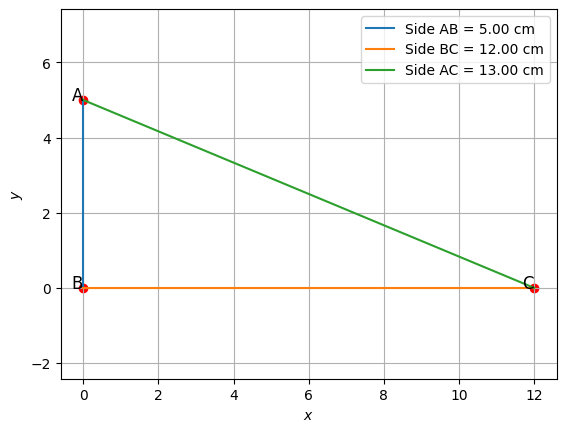
\includegraphics[width=\linewidth]{plots/plot.png}
		\caption{}
       		\label{graph}
    	\end{figure}

	


  
\end{document}


